\documentclass[journal,onecolumn]{IEEEtran}

\usepackage{cite}

% *** GRAPHICS RELATED PACKAGES ***
%
\ifCLASSINFOpdf
  \usepackage[pdftex]{graphicx}
  % declare the path(s) where your graphic files are
  % \graphicspath{{../pdf/}{../jpeg/}}
  % and their extensions so you won't have to specify these with
  % every instance of \includegraphics
  % \DeclareGraphicsExtensions{.pdf,.jpeg,.png}
\else
  % or other class option (dvipsone, dvipdf, if not using dvips). graphicx
  % will default to the driver specified in the system graphics.cfg if no
  % driver is specified.
  \usepackage[dvips]{graphicx}
  % declare the path(s) where your graphic files are
  % \graphicspath{{../eps/}}
  % and their extensions so you won't have to specify these with
  % every instance of \includegraphics
  % \DeclareGraphicsExtensions{.eps}
\fi

% *** SPECIALIZED LIST PACKAGES ***
%
\usepackage{algorithmic}

\usepackage{array}

% *** SUBFIGURE PACKAGES ***
%\ifCLASSOPTIONcompsoc
%  \usepackage[caption=false,font=normalsize,labelfont=sf,textfont=sf]{subfig}
%\else
%  \usepackage[caption=false,font=footnotesize]{subfig}
%\fi
% subfig.sty, written by Steven Douglas Cochran, is the modern replacement
% for subfigure.sty, the latter of which is no longer maintained and is
% incompatible with some LaTeX packages including fixltx2e. However,
% subfig.sty requires and automatically loads Axel Sommerfeldt's caption.sty
% which will override IEEEtran.cls' handling of captions and this will result
% in non-IEEE style figure/table captions. To prevent this problem, be sure
% and invoke subfig.sty's "caption=false" package option (available since
% subfig.sty version 1.3, 2005/06/28) as this is will preserve IEEEtran.cls
% handling of captions.
% Note that the Computer Society format requires a larger sans serif font
% than the serif footnote size font used in traditional IEEE formatting
% and thus the need to invoke different subfig.sty package options depending
% on whether compsoc mode has been enabled.
%
% The latest version and documentation of subfig.sty can be obtained at:
% http://www.ctan.org/tex-archive/macros/latex/contrib/subfig/

% *** PDF, URL AND HYPERLINK PACKAGES ***
%
\usepackage{url}

% correct bad hyphenation here
\hyphenation{op-tical net-works}

\begin{document}

\title{Volunteers in the Clouds: an Architecture for Low Cost and
  Potentially Massive Distributed Evolutionary Computation} 

\author{Juan-J.~Merelo*$^1$, Mario Garc\'ia-Valdez$^2$, Pedro A. Castillo$^1$, Pablo Garc\'ia-S\'anchez$^1$
\thanks{Manuscript submitted for review on \today.}%
\thanks{$^1$Dept. of Computer Architecture and Technology and CITIC University of Granada}%
\thanks{$^2$Dept. of Graduate Studies at Instituto Tecnol\'ogico de Tijuana}%
\thanks{E-mail addresses: {\tt jmerelo@ugr.es}, {\tt
    mario@tectijuana.edu.mx}, {\tt pacv@ugr.es}, {\tt pablogarcia@ugr.es}}%
\thanks{*Corresponding author.}%
}

\maketitle

\begin{abstract}
Volunteer computing is used routinely in science and industry, but it
still has a long way to go if it is going to become a mainstream technology in the
same way the cloud technologies in general have. The lack of general purpose and open source tools
with analytics built in could be one of the reasons why this is so, as
well as the lack of proofs of concept. That is why in this paper we
present NodIO, a client-server architecture for distributed
evolutionary algorithms, written entirely in JavaScript, which needs
minimal server support to work and is able to support persistent,
asynchronous, distributed evolutionary algorithms running in the
browser. The architecture, along with some initial results on the expected performance and scaling
behavior is presented. We also use the algorithm data to  %[Pedro] I don't understand what "the algorithm analytics" stand for???
% data - JJ
find out what kind of patterns the user behavior follow and try to fit them to some statistical distribution.
\end{abstract}

% Note that keywords are not normally used for peerreview papers.
\begin{IEEEkeywords}
Evolutionary algorithms, evolutionary computation, distributed computing, internet computing,
social networks, volunteer computing, metacomputing. 
\end{IEEEkeywords}


%---------------------------------------------------------------
\section{Introduction}

\IEEEPARstart{N}{owadays} there is a big and increasing number of
distributed evolutionary computation software frameworks available on
the market, usually as open source systems \cite{Parejo12Survey}. Most of these systems have %FERGU: añadida referencia
two features: they are {\em desktop} applications, that is, they must
be compiled or run directly on the operating system layer and, second,
they assume that the nodes that are going to run the system are under
your control or at least you have access to them.

There is, then, space for systems that do not have any of these %[Mario] these assumptions? [JJ] OK
assumptions, such as the one presented in this paper, which will be
provisionally named {\sf NodIO}. NodIO is first an application that
runs in two tiers, a server and a client, the latter  can be possibly
run on a  % [Pedro] Both the server and the client in browsers?
          % different browsers as I understand? [JJ]  No, server in
          % server, client in browser, although there's nothing that
          % can't be done in a browser. 
browser. As such, it can be run in any computer that loads the web
page where the client is embedded, including many over which%[Mario]Quitar el possibly?   [JJ] Done
the scientist has no control. 

Some time ago, our group faced the problem of diminishing funds for
buying new     % [Pedro] This sentence is so so long. I would split it
               % in two sentences. [JJ] Done.
hardware. This was aggravated by the increasing maintenance costs and extended downtime resulting from the continuous failures of existing clusters.
Considering this, we leveraged our experience in the design of web
applications, including JavaScript, since their inception and other
volunteer and 
unconventional distributed evolutionary computing systems, and we 
decided to design and release a new free framework that would allow anyone to
create a volunteer distributed EC experiment using cloud resources as
servers and browsers as clients.

This kind of systems must solve a series of issues before even starting to %FERGU: cambiado el "these systems" porque parecía que hacía referencia a "los anteriores" 
measure their performance; these issues are related to security as well as
safety, which introduces a {\em social} aspect to the design of a
computing system that makes it a {\em techno-social system}
\cite{vespignani2009predicting}. In this paper our intention is to
present the {\sf NodIO} framework and analyze it from two different
angles: the purely technical angle, including the decisions that went
into its features, and the social angle, to account on how the persons
that voluntarily choose to enter the web page that runs the system
determine its performance and how it can be modeled and, eventually,
predicted. 

The rest of the paper is organized as follows: Next we present the
state of the art (Section \ref{sec:soa}) in web-based distributed 
computation systems along with attempts to predict and model its behavior. %FERGU: El IEEE es americano
Then, a detailed description of the proposed system is presented 
in Section \ref{sec:description}, followed by the experiments and 
obtained results in Section \ref{sec:experiments}.
Finally, conclusions and future work are presented in Section \ref{sec:conclusion}. 


%---------------------------------------------------------------
\section{State of the art}
\label{sec:soa}

The web used as a resource for distributed computing has a
long history, and almost since the beginning it was used for 
evolutionary computation even before JavaScript was
introduced as a browser-based scripting language in 1997. Before that
time other technologies,
 including Flash animations and VBScript, ActiveX or Java applets were
used; for instance, Java was pointed out in \cite{soares1998get} as a ``language for
internet'', providing some advantages such as multi-architecture compatibility or 
security mechanisms and was proposed in \cite{chandy1996world} as the
basis for the creation of a world-wide peer to peer system using Java
compiled programs. The ATLAS system
\cite{Baldeschwieler:1996:TIG:504450.504482} also used Java together
with another language called Cilk; all these papers indicated that
the introduction of an architecture-independent system such as the
Java virtual machine opened the doors for ultrascale, Internet-wide,
metacomputers. This paper also establishes the desirable features of
any {\em global computing} infrastructure, that can also be applied to
distributed evolutionary computation experiments that rely on
volunteer computing: scalability, heterogeneity, fault tolerance,
adaptive parallelism, safety, anonymity, hierarchy, ease of use and
reasonable performance. Of all these, probably {\em hierarchy}, that
is, the capability of using preferentially resources in the same
organization could be either disregarded or included in adaptivity,
leaving us with eight desirable properties. 

Fulfilling these properties could be achieved using any of the
languages, and associated technologies, mentioned above, provided that the user had
installed the required virtual machine plugin first, but with the advantage of
providing a single and universal way of accessing resources via an
URI, something that is not guaranteed using desktop
applications. Baratloo et al. tried in 1996 to create a system with
the aforementioned qualities called {\em Charlotte}
\cite{baratloo1996charlotte}. This system, which implemented a
distributed shared memory, was inspired by previous work
on parallel computing systems PVM and MPI and solved most issues by
using the Java virtual machine embedded in the browser,
which provides
security to the user, uniformity of computing environment
independently of the operating system and access to a common data store in the
server. Since the virtual machine is a sandbox, it is safe to the user
and running a compiled bytecode guarantees a certain level of
performance. 
 Other issues such as scheduling, which are related to adaptive
 parallelism, are solved on the server. This 
paper was later extended and published in a journal in 1999
\cite{baratloo1999charlotte}, but it is interesting to note that
already in the early stages of the web the possibility of
browser-based distributed computing was already researched. 

Other systems, like JET, proposed by Soares et
al. \cite{soares1998get}, also used Java. JET supports 
the execution of parallel applications over the Internet and features
a comprehensive statistics collection subsystem, allowing its use for science,
since it allows the collection of algorithm analytics by the
experiment designer, unlike the other systems mentioned
above. Other proposals contemporary to Jet, such as SuperWeb
\cite{alexandrov1997superweb} are roughly a translation of classical
distribution techniques, with complicated architectures that include
brokers for resource discovery. It is focused, however, in solving the
issues involved in browser-based computing and also in making a system
that is able to work across different classes of computers, mentioning
SPARCstations and PCs with Windows-95. Interestingly enough, this
paper incorporates a discussion on the economic model, paving the way
for the for-profit distributed computing systems that later on
arose. On the other hand, the potential for volunteer computing using
browsers was realized 
later on \cite{sarmenta-bayanihan} as well as the potential for
mischief of users with code in their hands
\cite{sarmenta-sabotagetolerance}. However, these early efforts by
Sarmenta once again used Java and not JavaScript, making this effort
less widespread.

The main problem with Java and all the other browser-embedded
technologies is that they are not {\em universal} in the
sense than an extra component, namely, the Java virtual machine, has
to be installed in the browser. JavaScript, however,
\cite{flanagan2006javascript} was introduced in 1997 as a
browser-embedded language and has, since then, become a set of standards
\cite{ECMA-262} that include the language and its components. Since
early on, it was adopted by the industry and also by scientists,
who used them for creating an EA on
the browser as early as 1998 \cite{jj-ppsn98}. 

JavaScript can be used either for unwitting
\cite{unwitting-ec} or volunteer
\cite{langdon:2005:metas,gecco07:workshop:dcor} distributed
evolutionary computation and it has been used ever since by several
authors, including more recent efforts \cite{Desell:2008:AHG:1389095.1389273,duda2013distributed,DBLP:journals/corr/abs-0801-1210} that even
used the client's GPU \cite{duda2013gpu} or create an object-oriented
framework for evolution in the browser \cite{EvoStar2014:jsEO}. Many other researchers have
used Java \cite{chong:1999:jDGPi} and others have gone away from the
server-based paradigm to embrace peer to peer systems
\cite{jin2006constructing,10.1109/ICICSE.2008.99,DBLP:conf/3pgcic/GuervosMFEL12}. These computing
platforms avoid single points of failure (the server) but, since they
need a certain amount of infrastructure installed to start, the
threshold to join them is much lower. 

Recent works propose the use of cloud computing services for the components of 
client-server distributed EAs. Cloud resources 
can reduce operational costs by outsourcing both hardware and software maintenance 
to the cloud provider. Another advantage is that they enable the provisioning of computing resources beyond what 
is available in most laboratories, allowing researches to 
scale algorithms at reasonable costs. Researchers have proposed the use of 
public clouds such as Amazon EC2 \cite{CloudScale}, Google App Engine\cite{di2013towards} 
and DropBox~\cite{mericloud}. The use of JavaScript to implement server side components, %FERGU: he puesto mejor el de revista en lugar del del CEC
gives software developers certain advantages in the cloud paradigm. JavaScript is a first-classe citizen
in most Platforms as a Service (PaaS) as many support the Node.js framework \cite{wood13:nodejs:paas}. Also many web services 
have native JavaScript libraries and use JSON for data interchange. Another advantage is that 
developers can use the same software tools for both client and server side development. 
Besides the advantages to deal with the same language in the full stack as previously mentioned, 
this also facilitates the interoperability of the exchanged data types.
%Ayuda con la mini conclusion FERGU: mira la última frase de arriba

In the work presented in this paper, JavaScript has been used throughout the full 
stack, which has the advantage of using the same lines of code for
writing an evolutionary algorithm for the
desktop or command line and browser clients, both based in the EC
library NodEO \cite{DBLP:conf/gecco/GuervosVGES14}. This saves time
when writing code and leverages %FERGU: qué diferencias hay entre NodIO y NodEO??
expertise acquired in the library itself. %FERGU: tienes info de LoC
                                %usadas para la sección experimental y
                                %justificar esta frase?
% Es el mismo código - JJ
%The proposed software has the advantage of full stack JavaScript
%development..

Javascript is also compatible with the functional programming paradigm \cite{Cousineau1998,MacLennan1990,Thompson1996}. 
According to \cite{swanresearch2015}, the benefits of using this kind of paradigm in 
metaheuristics optimization allows an improvement in communicability, 
reproducibility, interoperability, automated assembly, knowledge engineering 
and efficiency. 

There have been relatively few efforts to analyze the
performance that can be obtained from these volunteer computing
experiments. 
There were some initial attempts to avoid the differences in performance
that could be obtained from volunteers  by making
the algorithm adaptive to the kind of resources allotted to it
\cite{milani2004online}, which is actually not such a big problem in
algorithms such as the EA that can easily be
parallelized via population splitting or farming out evaluations to all
the nodes available. Lately, several approaches have focused on the
fault-tolerance of volunteer algorithms
\cite{gonzalez2010characterizing} which can, of course, be studied in
a more general distributed computing context
\cite{nogueras2015studying} or including it in a more general study of the
performance of the EA itself
\cite{DBLP:journals/gpem/LaredoBGVAGF14}. 

%Mario: Estaba pensando que otra justificación muy fuerte para el uso de JS sobre plug-ins 
%ha sido la seguridad ya que estos presentan otra fuente de vulnerabilidad. Para complicar las cosas a veces (Flash, ActiveX) 
%son tecnologías cerradas y propietarias. Por lo menos creo que esas
%fueron las razones que se dieron para eliminar a Flash del iPhone.
% [JJ] Escribe algo...

As far as we know, this paper presents one of the few experiments that
uses computational 
resources that are as dissimilar as smartphones and powerful laptops
or desktop computers in a research center. The methodology used to
gather resources and the algorithms used will be described next, as
well as the results obtained with the setup.

%El último párrafo podría ser más preciso. Es el único experimento que utiliza recursos heterogeneos
%empleando las tecnologías estándar (JavaScript, JSON, Cookies, etc.) mencionadas previamente.

%Si no se extiende mucho se podría también hablar de la conexión con Cloud Computing,
%se discuten las ventajas de utilizar Javascript para acceder a recursos donados por voluntarios
%pero falta hablar de como se explotaría el recurso Cloud. Lo digo por el titulo de Volunteers in the Clouds. Tal vez
%se deba hablar de la posibilidad de escalar los sistemas a bajo costo
%o según la demanda.

% Si te animas, propón un párrafo - JJ
% Ok, lo escribo. - Mario
% Voy escribiendo algo de HTML5 y Web Workers?, no necesariemente para
% esta sección. 
% Para la intro o esta sección - JJ


On the other hand, measuring performance of the resulting metacomputer
involves understanding the dynamics of this kind of systems. Initial
work was done for peer to peer systems by Stutzbach et
al. \cite{stutzbach2006understanding} and extended to volunteer
computing by Laredo et al. \cite{churn08,laredo2008rcp}. But the raw material of
volunteer computing, number of users and the time spent in the
computation in browser-based volunteer computing experiments, have only been studied in a limited way in
\cite{DBLP:journals/gpem/LaredoBGVAGF14} on the basis of a single
run. Studies using volunteer computing platforms such as SETI@home
\cite{javadi2009mining} found out that the Weibull, log-normal and Gamma distribution
modeled quite well the availability of resources in several clusters
of that framework; the shape of those distributions is a skewed bell
with more resources in the {\em low} areas than in the high areas:
there are many users that give a small amount of cycles, while there
are just a few that give many cycles. This is in concordance with the
results obtained in \cite{agajaj}. Our initial tests indicate that
this kind of distribution might be the most appropriate to describe
user participation in several different metrics. However, in this
paper we will perform different experiments in different setups and
will try to come up with a more precise model. Next we describe the
system itself. 

%---------------------------------------------------------------
\section{Description of the system}
\label{sec:description}

In general, a volunteer-based distributed evolutionary computation
system based on the browser is simply a client-server architecture
whose client is, or can be, embedded in the browser via JavaScript. 

% [Pedro] desde el abstract no se había nombrado "NodIO". 
% Creo que en este párrafo debería introducirse, principalmente el nombre.
% Añado una frase presentándolo:
% [Mario] Nota: se menciona también en el segundo párrafo de la
% Introducción.
% OK [JJ]
In this sense, in this paper we propose {\sf NodIO}, a cloud or metal based 
volunteer computing system, whose architecture
has been developed using JavaScript on both the client and server sides.
All parts of the system are free and available with a free
license from \url{https://github.com/JJ/splash-volunteer}.
Thus, {\sf NodIO} architecture has two tiers:\begin{enumerate}
\item A REST server, that is, a server that includes several remote %remote requests suena raro, propongo algo como: remote procedures o web interfaces   
  requests for storing and retrieving information (the CRUD cycle:
  create, request, update and delete) from the server. The information
  is of two kinds: {\em problem} based, that is, related to the
  evolutionary algorithm such as {\tt PUT}ing a chromosome in or {\tt
    GET}ing a random chromosome from it, and {\em information} related
  to performance and state of the experiments. It also performs logging
  duties, but is basically a very lightweight and high performance
  data store \cite{jj:idc:lowcost}. 
  %The information is of two kinds: Problem Based y ¿Cual otra?
  %¿Logging? No se entiende bien. ¿Podría ser problem domain?   
% info. Añadido [JJ]
  The server has the capability to
  run a single experiment, storing the chromosomes in a data structure
  that is reset when the solution is found. 
\item A client that includes the evolutionary algorithm as 
  JavaScript code embedded in a web page that displays graphs and some
  additional links and information on the experiment. This code runs
  an evolutionary algorithm {\em island} starting with random
  population and sending, every 100 generations, the best individual
  back to the server (via a {\tt PUT} request) and requesting a random
  individual from the server (via a {\tt GET} request). Apart from
  these constants, the algorithm can be run in many different ways:
  stopping when solution is found or, as we have done in this paper,
  using WebWorkers, which run in the background even if the webpage or
  browser tab with the experiment is not currently on focus.  
\end{enumerate}

Figure \ref{fig:system} describes the general system architecture and
algorithm behavior. Different web technologies, such as JQuery or chart.js have
been used to build the elements of the system. 
%FERGU: Mario, explica en el texto de abajo qué es winston en la figura también. 
%Vamos, que todo lo que salga en la figura tiene que ir en el texto en alguna parte :)
% [Mario] Ok voy a explicar la figura. Quería saber primero su opinión tal vez se les hacía mucho detalle.
% Creo que esta figura va mejor en la sección donde hablamos de
% webworkers. La anterior era más adecuada como visión general. [JJ]
\begin{figure}[!t]
\centering
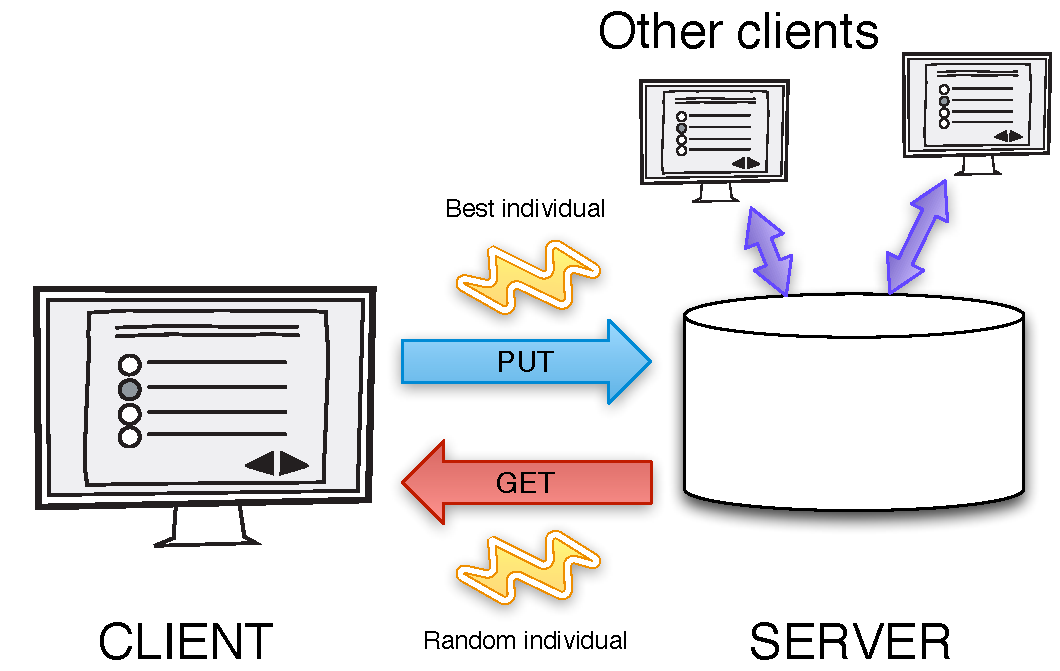
\includegraphics[width=4in]{img/system.pdf}
\caption{Description of the proposed system. Clients execute a JS EA
  in the browser, which, every 100 generations, sends the best
  individual and receives a random one from the server. }  
\label{fig:system}
\end{figure}

The researcher only has to change a function to solve a different
problem, in this case the classical Trap function \cite{Ackley1987} has been 
used. JavaScript is a functional language and declaring a different
function and handing at the creation of the algorithm object, called
{\tt Classic} is the only change needed to work with a different
problem. Let us see how this system addresses the different challenges
outlined in the State of the Art (Section \ref{sec:soa}):\begin{itemize}
\item {\em Scalability} is provided via the use of a lightweight and
  high-performance, single-threaded, server based in NodeJS and
  Express.js. Although this single server is a bottleneck since it
  will eventually saturate, the fact that it runs as a single thread
  allows the service of many requests. In fact, a limit with the
  number of simultaneous requests will be reached, but so far it has
  not been found, unlike what we found in our previous systems, DCoR,
  \cite{gecco07:workshop:dcor}, which had a low scalability.
\item The system is {\em heterogeneous} since it does not need any
  performance, operating system or even browser requirement: anyone
  visiting the page, even from mobile devices, can load the algorithm. 
\item {\em Fault tolerance} is always an issue, and in this case, the
  single point of failure would be the server: the system, as such,
  would break down if the server fails. However, the individual
  islands in every browser would continue running, and having access
  to just one of them would allow the local algorithm to proceed. In
  fact, the island does not need the server to run: it runs locally if
  needed, with the only exception that it is obviously unable to
  communicate with the rest of the islands.
\item {\em Adaptiveness} is achieved simply through autonomous
  operation of every individual island and no synchronization
  mechanism. The islands in the system are, in fact, unaware of each
  other, communicating only through the server.
\item Since the algorithm is run on the browser, {\em safety} is
  achieved through its sandbox mechanisms. The user is thus assured
  that there is no unsafe access either to their local files or even
  to more resources that the browser should be allotted.
\item Running the algorithm is just a matter of loading the page,
  which means that operation is totally {\em anonymous}. For the same
  reason, {\em ease of use} is optimal, being as easy as simply
  clicking on an URL and available to anyone with access to a browser.
\item {\em Reasonable performance} is not ensured. In fact, we should
  make sure that there is a reasonable amount of clients over which
  the performance achieved is bigger than what you would obtain in
  your own desktop system. If that is not done, it is a pointless
  academic exercise.
\end{itemize}

This last point is what we will try to prove next.

%---------------------------------------------------------------
\section{Experiments and obtained results}
\label{sec:experiments}

\begin{figure}[!t]
\centering
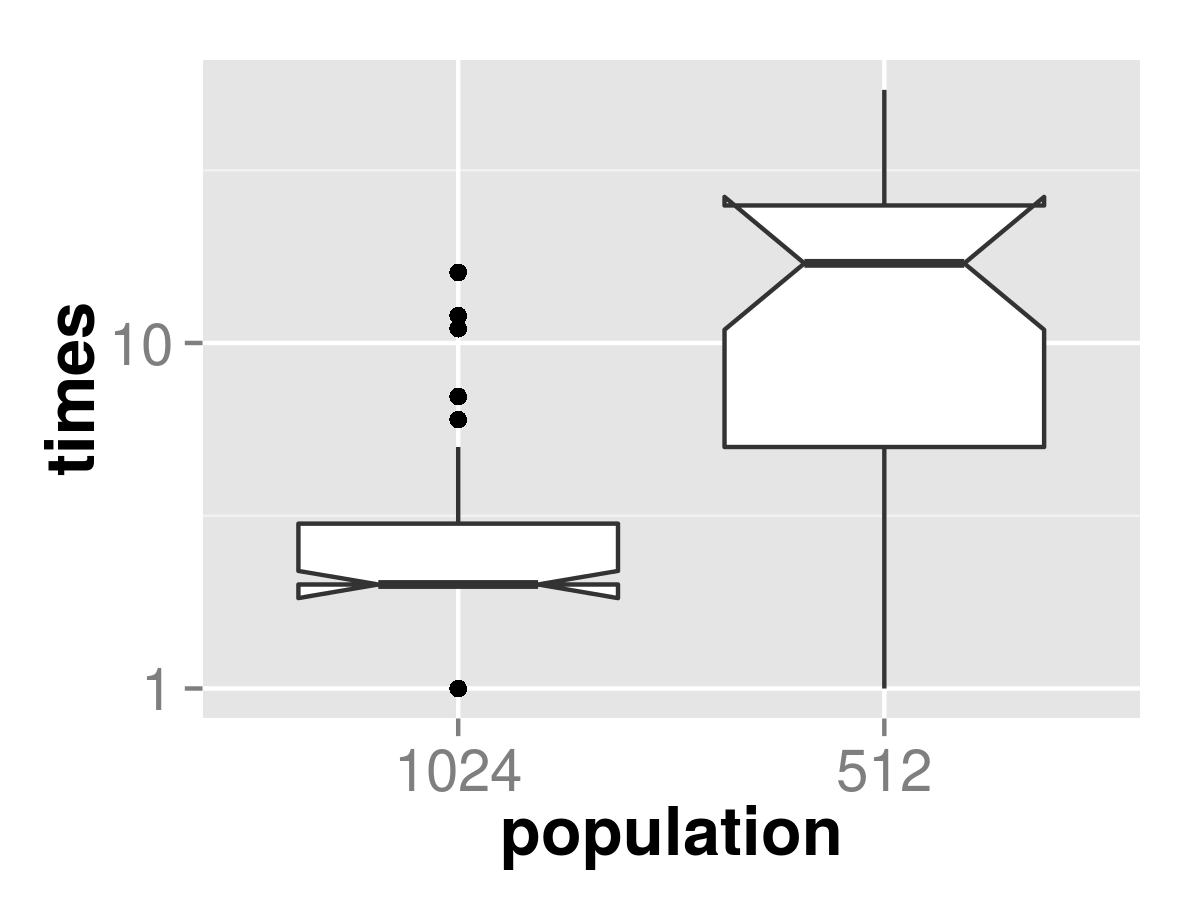
\includegraphics[width=12cm]{img/baseline-times.png}
\caption{Comparison of time to solution for the baseline system, using a {\tt
    node.js} client, for different population sizes. They only compare on
runs in which solution has been found.}
\label{fig:baseline}
\end{figure}
First we establish the baseline performance by running the
evolutionary algorithm in a desktop client written using NodEO, 
%FERGU: es NodEO o NodIO? Quito el \sf, por cierto, que queda feo
%Por qué usamos NodEO aquí y no NodIO, vamos a compararlos? 
%Qué diferencias hay entre los dos? (ponerlo en el SOA)
%[Mario] Creo que es NodEO y NodIO fué mi error.
the node.js evolutionary algorithm library. This experiment tries to 
%FERGU: quitar el "the node.js evolutionary algorithm library", si ya lo hemos dicho
%o explicarlo mejor: "the basic js library we have used as base to built NodIO", por ejemplo
find the solution to the 40-trap function with parameters $l=4, a=1,
b=2, z=3$, a population size equal 512, which was found in previous
experiments to be the correct one for finding the solution 95\% of the
%Fergu: cita a esos experimentos?
time. The algorithm was run until the solution (a string with all
ones) was found or five millions evaluations had been performed. It
took around a minute, on average, that is $68.9694$ seconds, to
perform the fifty runs. In this experiment only 33, that is, 66\% were
successful. The experiments were repeated for population $p=1024$,
with success rate upgraded to 100\% and average duration $3.46$
seconds. Results for these two experiments 
are shown in Figure \ref{fig:baseline}.

These two experiments establish first a baseline result, which will
depend on the population. The volunteer computing experiments that we
will describe next do not and can not have the same conditions, but
the baseline is that if they eventually take longer than a basic
desktop, their interest will be purely academic. We will try and
prove next that that target performance can be achieved by carrying
out several experiments in different conditions.

\subsection{Volunteer evolutionary computation: first experiments and results}

Initial experiments were set up using the OpenShift
Platform-as-a-Service, which provides a free tier within which this
experiment could be performed. That way, and as required, the hardware
and cloud cost for this experiment were zero. Experiments were
announced through a post in Twitter and other social networks, and
results were published here \cite{DBLP:conf/gecco/GuervosG15}. For the
purpose of this paper, we repeated the announcement several times
through the months of April and then by the beginning of August. All
in all, we have the set of runs with the characteristics shown in
Table \ref{tab:runs}. In general, every experiment took several
days. No particular care was taken about the time of the announcement
or the particular wording. Every {\em experiment} consisted in running
until the solution of the 40-trap problem was found. When the correct
solution was sent to the server, the counter was updated and the pool
of solutions reset to the void set. No special care was taken to wait
until all clients had finished, thus it might happen that, in fact,
the islands running in the browser {\em spill} from one experiment to
the next. However, previous experiments have proved that the influence
of these islands in the next experiment is, in fact negligible.
%
\begin{table*}d
\caption{Characteristics of the volunteer computing initial runs. \label{tab:runs}}
\begin{center}
\begin{tabular}{l|rr}
\hline
Date & \# experiments & Different IPs \\
\hline 
April 4th 4/4 & 57 & 191 \\
April 24th 4/24 &  231 & 559 \\
July 31th 7/31 & 97 & 179 \\
\hline 
\end{tabular}
\end{center}
\end{table*}
%
\begin{table*}
\caption{Summary of time per run, number of IPS and number of {\tt
    PUT}s per IP in the initial runs. \label{tab:summary:os}}
\begin{center}
\begin{tabular}{l|cccccc}
\hline
Date & Median \#IPs & Max \#IPs & Median time (s) & Median \#{\tt PUT}s & $<$ 69s & $<$ 3.46s \\
\hline 
4/4 & 5 & 16 & 2040 & 18 & 14.29\% & 5.36\% \\
4/24 &  5 & 29 & 732 & 11 & 47.39\% & 3.91\% \\
7/31 & 5 & 14 & 260 & 23 & 27.08\% & 1.04\%  \\
\hline 
\end{tabular}
\end{center}
\end{table*}
%
The table shows that every run included more than 50 experiments. The
number of different IPs intervening in them varied from more than one
hundred to more than five hundred in the second experiment. 

A summary of the results of each run is also shown in Table
\ref{tab:summary:os}. This table shows the median number of IPs
intervening in each experiment,  median of the time needed
to finish the experiment, median number of HTTP {\tt PUT}s per IP, and
then two columns showing the percentage of experiments that took less
than the two baseline experiments shown in the introduction to this
section. The first striking result is that in all cases, 50\% of the
experiments involved 5 or less IPs. This is consistent with results
found previously \cite{DBLP:conf/gecco/GuervosG15} which found 6 to be
the usual number of IPs that participated in an experiment. 

\subsection{{\sf NodIO-W$^2$}, a WebWorker-based architecture}

\begin{figure}[!t]
\centering
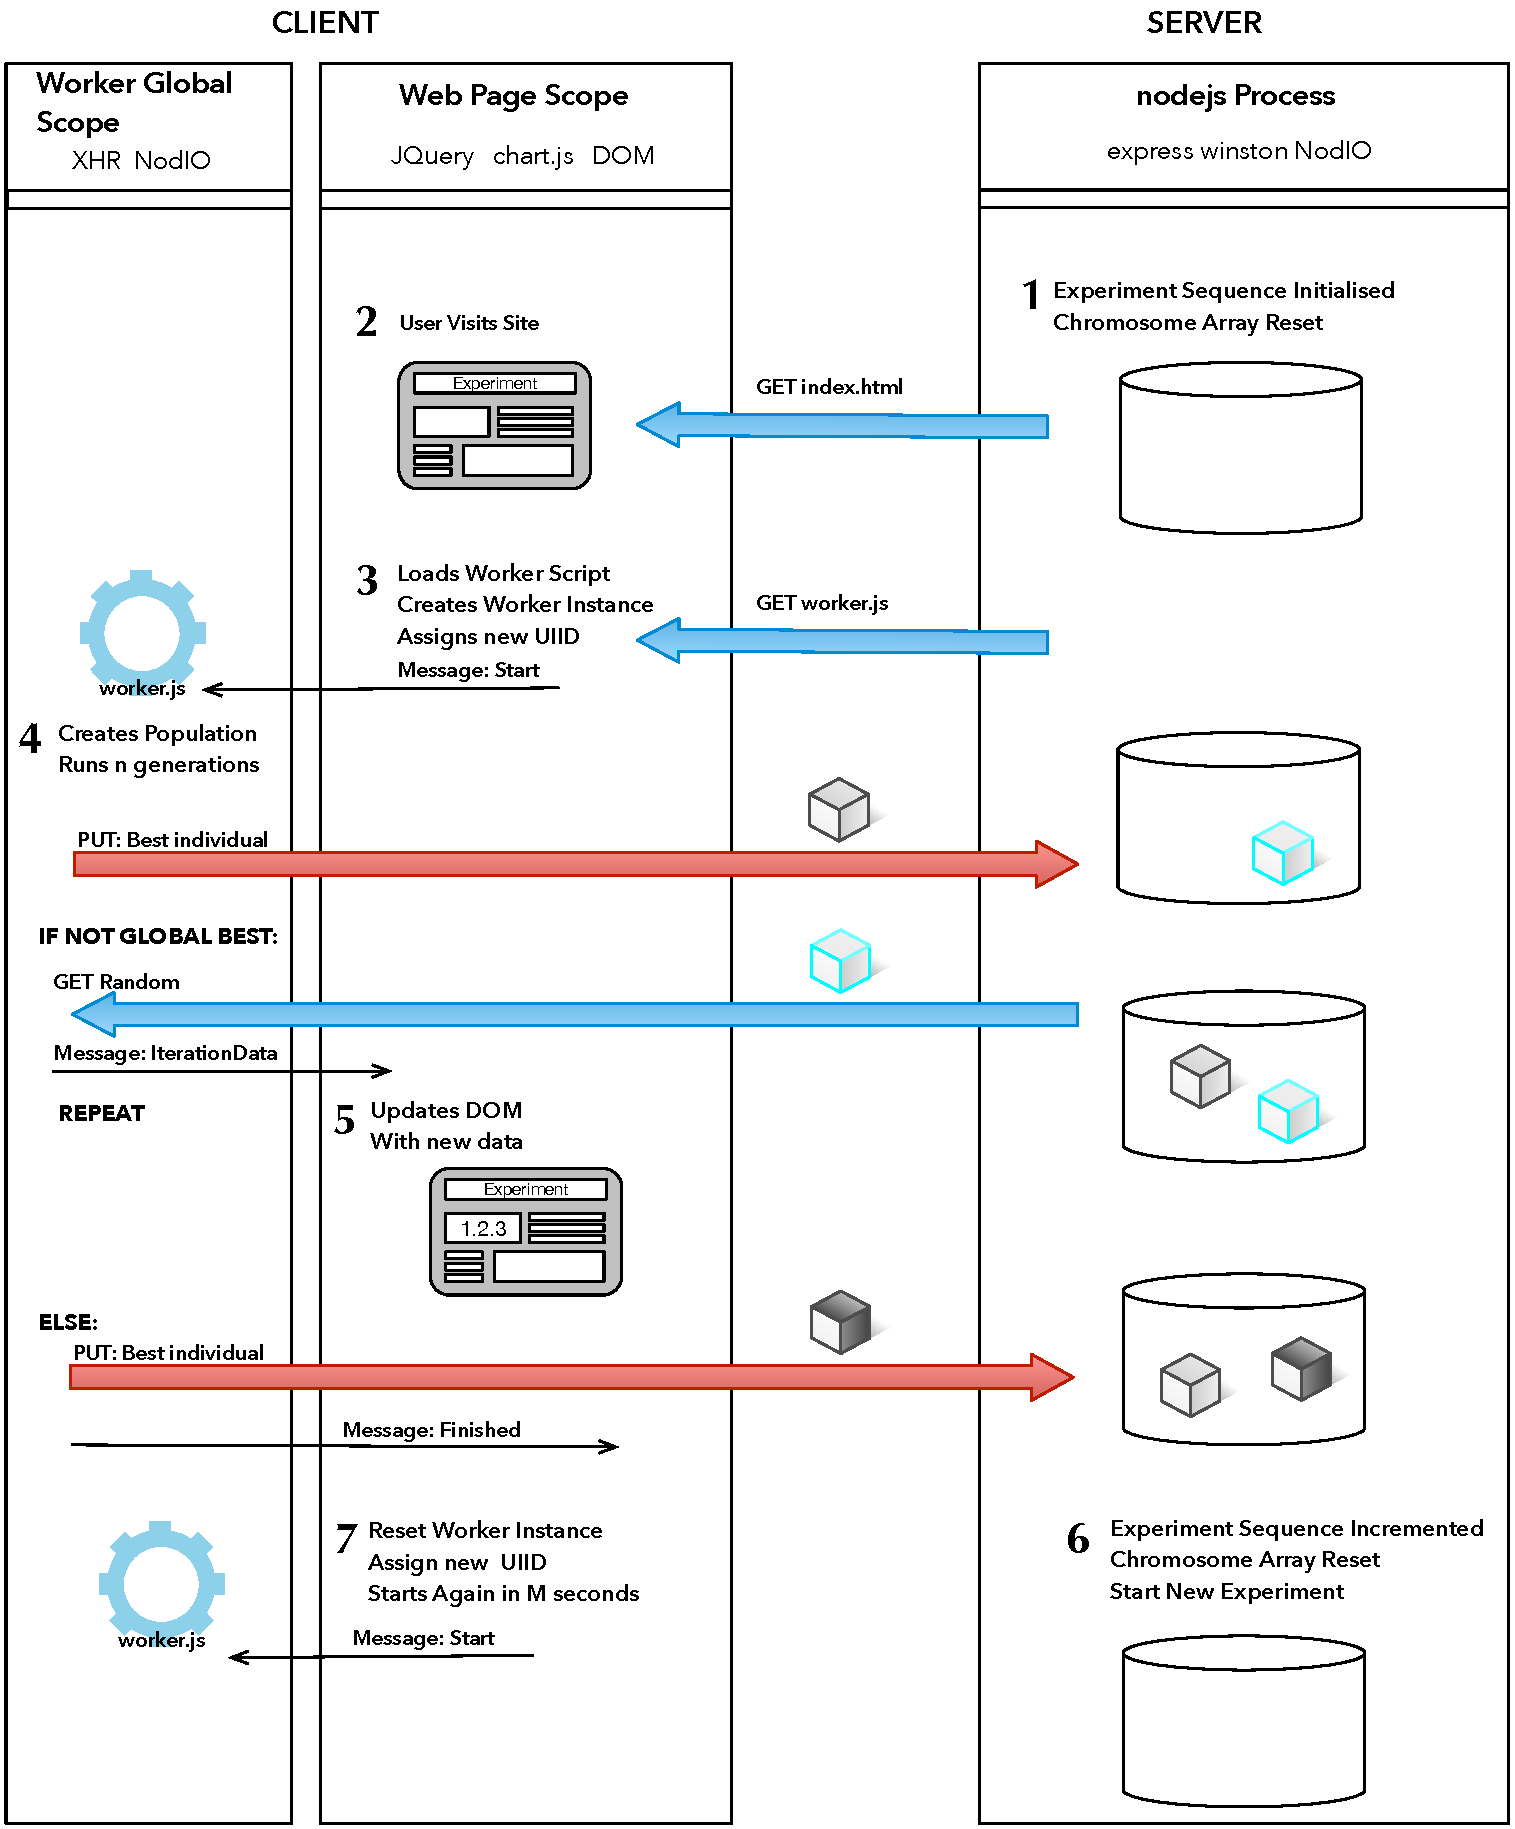
\includegraphics[width=4in]{img/Algorithm.pdf}
\caption{Description of the W$^2$ version of {\sf NodIO}. In this
  version, clientts use WebWorkers to run the evolutionary algorithm,
  with two of them per browser.}  
\label{fig:system:w2}
\end{figure}

%---------------------------------------------------------------
\section{Conclusion}
\label{sec:conclusion}

The conclusion goes here.


%---------------------------------------------------------------
% use section* for acknowledgment
\section*{Acknowledgment}

This work has been supported in part by TIN2011-28627-C04-02 and
TIN2014-56494-C4-3-P (Spanish Ministry of Economy and Competitivity),
SPIP2014-01437 (Direcci{\'o}n General de Tr{\'a}fico) and PYR-2014-17
GENIL project (CEI-BIOTIC Granada). We would also like to thank the
anonymous reviewers of previous versions of this paper who have really helped us to improve
this paper (and our work) with their suggestions.


\bibliographystyle{IEEEtran}
\bibliography{geneura,volunteer,javascript,ror-js,GA-general}

\end{document}
%%% Local Variables:
%%% ispell-local-dictionary: "english"
%%% End:
